Matrix Multiplication is a central operation in algorithms that are used every day now. E.g., training a model in Machine learning, displaying sharper images in Computer Graphics, predicting weather patterns in Scientific Computing, analysis of Social Network relations, studying cache designs in Computer Architecture, benchmarking the speed of a Supercomputer are a few important examples where matrix multiplication is employed. Improving the speed of computation of matrix multiplication has been the focus of mathematicians and computer scientists for many decades. Algorithmic improvements that yield lesser number of multiply-add operations~\cite{huss1996implementation}, improvements in scheduling of those operations to yield lesser number of memory accesses to the slow memory in modern computing systems with hierarchical memory~\cite{low2004api,van1997summa}, provisioning of dedicated hardware for simultaneous execution of several such operations form the broad spectrum of developments~\cite{10.1137/140993478}. Orthogonally, researchers have created abstractions and tools for developers to {\em quickly} produce fast matrix multiplication implementations: dedicated APIs for matrix multiplication in library-based development environment~\cite{MKL,Alpatov1997PLAPACKPL,goto2008high,choi1992scalapack,anderson1999lapack,libflame}, compilers to effectively map the operations to underlying hardware~\cite{ikarashi2022exocompilation}, and programming systems to abstract the specification of computation from orchestrating the computation on underlying (often) complex hardware~\cite{ragan2013halide}. This paper focuses on various factors 
 involved in system development ---development to deployment on specific systems--of matrix multiplication in an attempt to understand the trade-offs involved. Specifically, on a variety of hardware, such as DNN accelerators, GPUs, x86- and Arm-based multicore CPU servers, performance characteristics at different scales within the system are considered: i) within a core: SIMD/vectorized and multithreaded codes, ii)across cores: shared-memory parallel programming models using Cilk, OpenMP tasks, iii) hybrid codes i.e. CPU+GPU including automatically generated codes. Latency, energy consumed, and  speed of code development are measured for single- and double-precision data to understand the tradeoffs of execution time vs. \{precision, energy consumption\}, precision vs. energy consumption, speed of code development vs. \{energy consumption, execution time, and precision\}. The goal is to help application developers make an informed choice of the workhorse (system with appropriate programming abstraction and tools) for deploying their applications, which have matrix- multiplication as the underlying kernel. 
 
Modern computing systems provision for parallelism within a core, across cores, across a host within the same compute node hosting one or more `devices' or accelerators, and across a host with multiple nodes. A single optimized implementation that delivers the same level of performance with system configurations of different parallelism levels is challenging.  Developers dedicate significant time and effort to optimize matrix multiplication kernels to squeeze out every ounce of performance from the hardware resources available. We create `reasonably' efficient implementations of matrix multiplication {\em quickly} with the help of a tool, D2P~\cite{hegde2019d2p}, that produces parallel code exploiting parallelism across cores and across hosts on multiple compute nodes. Furthermore, D2P provisions for exploiting parallelism within a core and in a node with host-device mode of computing. This {\em elastic} parallel code is created from a specification, which we develop assuming dense matrix computation and a recursive divide-conquer (non-Strassen) matrix multiplication algorithm. A noteworthy feature of the elastic code is that the recursion base case is left empty to allow for optimized kernels to be plugged-in. Consequently, we plug in hand-tuned, optimized kernels (CUDA, AVX, Arm Neon, locality-optimized) and augment to create efficient, performance portable matrix multiplication implementations quickly. It is important to note that the development of hand-tuned optimized code is a one-time effort (often available) and 
 plugging-in and deploying augmented code on different systems is relatively easier.

 
%Therefore, To make the most of the underlying hardware capabilities, they employ SIMD parallelism, which includes the AVX and AVX2 instruction sets. They also use parallelizing constructs to optimize the performance of each core. 
%Better optimization requires in-depth analysis and profiling to comprehend trade-offs between latency, cost, energy consumption, and development speed.
% Gap?
%Our focus is on addressing the gap i.e., the need for a comprehensive analysis of the various aspects mentioned earlier.

Figure~\ref{fig:1} shows performance comparison of the augmented code 
 (indicated as hybrid code) and native CUDA-C code for multiplying two matrices. The hybrid code is a mix of MPI+Cilk+CUDA-C code. Interestingly, we see that in a compute node with multiple GPU cards, native CUDA-C implementation executes slower compared to the hybrid code. 
% Profiling details showed that the hybrid multi-GPU CUDA implementation spent only 27.5\% on kernel execution and the rest of 72.5\% of execution time on memory transfer. In contrast, the Native Single GPU and Native Multi-GPU implementations spend 98\% of their execution time on kernel execution and only 2\% on memory transfer. This large difference in time allocation explains why the hybrid code runs faster.
Performance counters from NVIDIA Nsight Compute indicate why the hybrid code performs better than the native code. The hybrid code records nearly 56 million DRAM active cycles, whereas the native code displays a much higher 9.54 billion cycles. The hybrid code also achieves better overall DRAM throughput (8.24\% versus 5.11\%) and memory throughput (21.95\% compared to 18.54\%). The  L1 cache throughput for hybrid code is higher than native code (43.32\% versus 37.08\%) but the hybrid code records comparatively lesser L2 cache throughput (4.09\% compared to 4.73\%). On the other hand, the registers per thread used for hybrid code (36) are lesser than native code (46), leading to greater parallelism . With slightly improved GPU occupancy (100.49\% versus 100.13\%), the hybrid code maximizes resource utilization more effectively, leading to faster execution and superior performance overall.
 We attribute this to the dynamic parallelism created in hybrid code, which is able to utilize the additional GPU resources efficiently. The recursion base cases (with CUDA kernels) in the hybrid code are independent tasks that get executed with the help of distinct MPI ranks. Note that both hybrid code (in the recursion base case) and native code use the same optimized CUDA kernel for matrix multiplication.
 This experiment shows that performance portability across multiple GPU cards is achievable with minimal programmer effort and surprisingly, tool-produced code can be faster than hand-optimized code. Is the performance portability free of cost? does data precision have an impact on performance and/or energy consumption? to understand these, we do a systematic analysis of the performance (execution time), development speed, and energy consumption of different flavours of matrix multiplication kernel implementations on a variety of systems, including Jetson Nano and cloud-based server instances. 
%We aim to identify each implementation's efficiency gains and tradeoffs across various hardware platforms. 
%In this study, we implement and conduct a thorough evaluation of hand-optimized versions, tool-generated implementations, and library-based solutions. 
%We test the performance, development speed, and energy consumption of SIMD codes such as AVX and AVX2, CPU-parallel codes like Cilk and OpenMP (OMP), CUDA for using the GPU card, and tool-generated hybrid parallel codes for various matrix sizes. We improve the recursive matrix multiplication algorithm by implementing multicore-specific Cilk and OMP parallelizing constructs. We used D2P to generate MPI and Cilk based hybrid code implementation by providing recursive algorithm specifications. The tool-generated code has the empty recursion base case, making it performance portable. We plug the hand-optimised AVX, AVX2 and CUDA codes into the base case.
The key contributions are:
%\begin{figure*}[h!]
%  \centering
%  \includegraphics[width=0.9\linewidth]{3dPlot.png}
%  \vspace{-0.8em}
%  \caption{Comparison of hand-optimized and tool-generated implementations of various programming models for both precisions.}
%  \label{fig:3d}
%\end{figure*}
\begin{itemize}
 
    \item We create specifications for recursive matrix multiplication algorithm and produce corresponding hybrid-parallel code.  
    \item We create a number of matrix multiplication implementations, including AVX256, AVX512, Arm Neon, OpenMP, Cilk, Jetson Nano, CUDA-C, Open BLAS-based, Tensorflow, and Pytorch based codes. We plug-in some of these codes into the recursion base case to produce efficient hybrid-parallel code. 
    \item we measure and analyze performance, energy consumed, precision and speed of development to understand trade-offs involved in multiplying matrices with different precision data, on systems at different scales, with different programming systems, under different energy consumption scenarios. 
\end{itemize}
\begin{figure}[H]
  \centering
  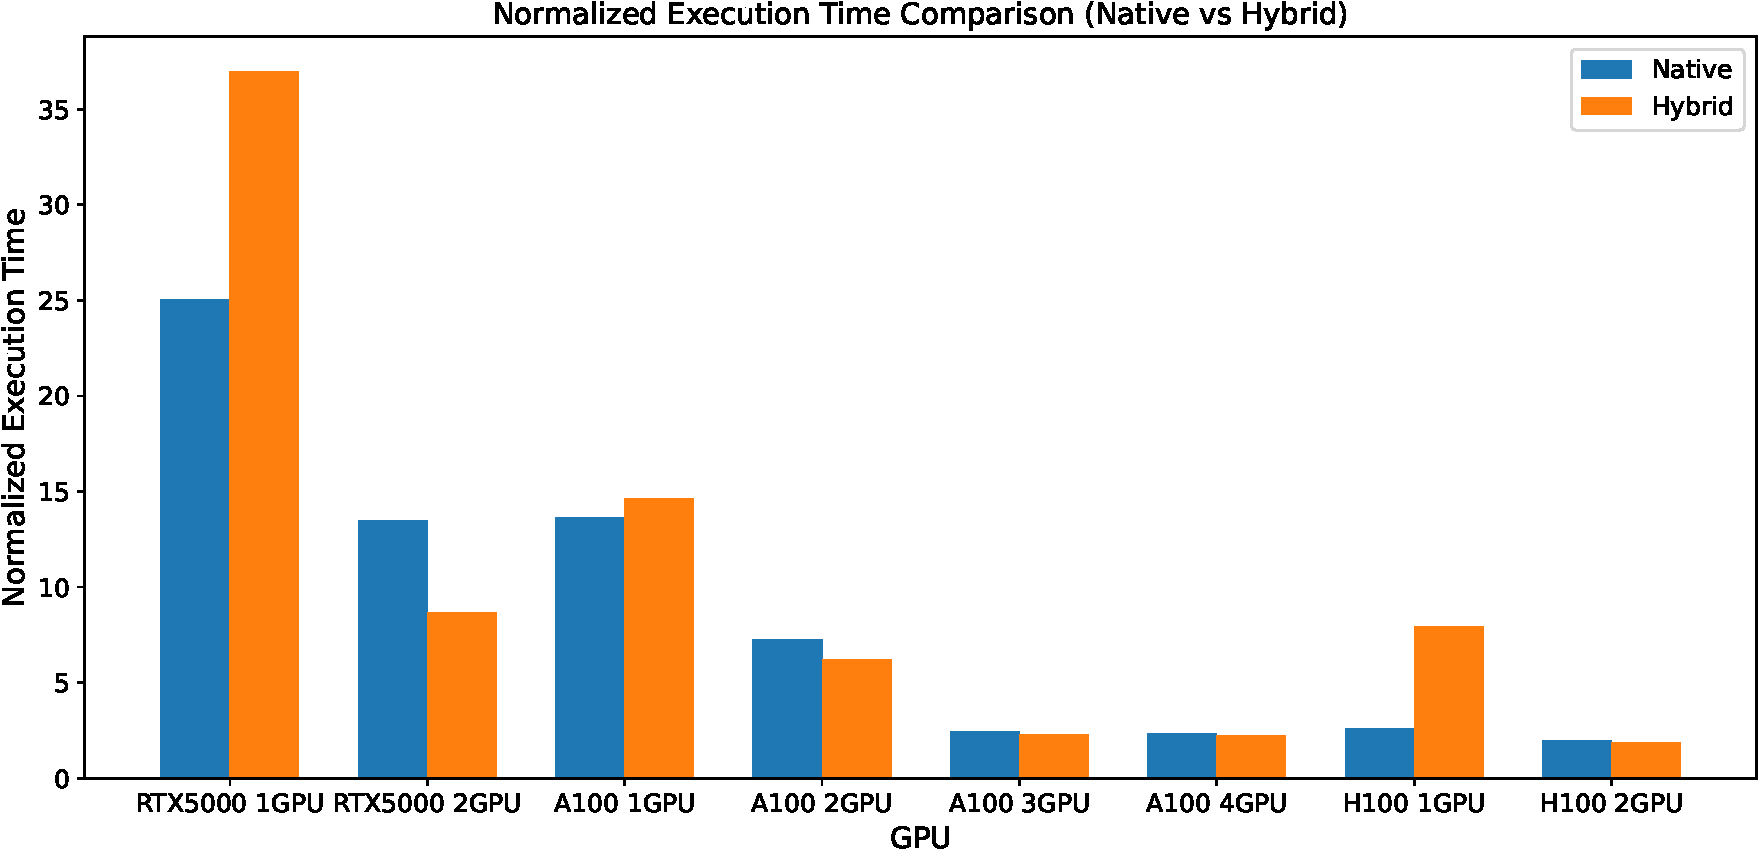
\includegraphics[width=1.0\linewidth, height=0.70\linewidth ]{Images/DiffHardware -crop.pdf}
  %\vspace{-0.8em}
  \caption{Native CUDA-C vs. Augmented CUDA-C comparison.}
  \label{fig:1}
\end{figure}

Tests across various systems show that overall, CUDA implementations executing on multiple GPUs deliver the best performance, offering the lowest latency. W.r.t. energy consumption of distributed workloads, surprisingly, codes executing on RTX5000 GPUs show that energy consumption get smaller with work distributed across available cards. In contrast, energy consumption increase with work distributed across available A100 and H100 GPUs.  As expected, increasing precision from single- to double- floating point computation is associated with longer execution time, which in turn is associated with increased energy consumption. The cuda codes on Jetson Nano w.r.t to performance %also take longer execution time and consume more energy for double precision than single precision. %jetson nano to a100, ARM and PNK, ARM VM and BM, omp & cilk on ARM
are 7.5x slower than RTX5000, 28.48x slower than A100 and 37.47x slower than H100. And w.r.t. energy consumption, Jetson Nano consumes 5.2x less energy than RTX5000, 10.49x less energy than A100 and 8.4x less energy than H100. 
Interestingly, for CPU Parallel codes like OMP and Cilk, OMP and Cilk on x86 are 1.4x and approximately 1.5x slower than runs on ARM for both single- and double- precision.
%Tests on AVX256 and AVX512 codes on RTX5000 show that AVX512 offers better performance and energy efficiency than AVX256 in both the precisions, w.r.t the Hybrid -AVX256 and -AVX512 codes, the performance is better for hybrid AVX512 but not energy efficient, and interestingly Hybrid AVX512 \& AVX512 codes deliver better performance than Native AVX256 \& AVX512  codes but energy consumption-wise Native codes are more energy efficient in both single and double precisions.
The SIMD codes on ARM, w.r.t. performance, are 1.9x slower than x86, whereas Hybrid SIMD codes on ARM are 20x slower than Hybrid SIMD x86 for single precision.
For double precision, Native SIMD on ARM is 4x slower than x86, whereas SIMD codes on ARM are 23.4x slower than Hybrid SIMD x86 for single precision.
A similar trend is observed in SIMD codes on ARM system w.r.t precision, additionally, native SIMD codes consistently perform better than Hybrid SIMD codes in single and double precisions. 
Also, ARM virtual machine instance SIMD codes are 1x slower than ARM Bare metal instances.
Tests on Colab for TPU and GPU usage using TensorFlow and PyTorch show that runs on TPU perform well when compared to GPU. TensorFlow code using TPU is faster than PyTorch using TPU for single and double precisions. In contrast, PyTorch GPU code is faster than TensorFlow GPU code.
Due to the limited access to performance counters on cloud-based instances and Google Colab, energy consumption was not measured.
%Experiments with different programming models on Arm-based and x86-based CPU-only servers, CPU-GPU servers with multiple GPU cards, and Jetson Nano demonstrate that CUDA implementations provide the lowest latency and are the most energy-efficient in a multi-GPU scenario with distributed work. 
%We see trade-offs across various CPU and GPU-based implementations demonstrated in the figure\ref{fig:1} below.
%We observe that double precision take more energy and are slower compared to single precision. We also see that using multiple GPUs can improve latency as the work can be disributed and computed simultaneously. we also observe that d2p+AVX512d seems to consume more energy than d2p+AVX256d for both single and double precision.
%Specifically, for double precision codes, we find that tool-generated code integrated with a manually optimised kernel on a multiple GPU setting performs better than native CUDA code in terms of latency, development speed, and energy consumption.
%We also see many other contrasting behaviors in figure \ref{fig:1}. A detailed discussion will be presented in the Result and Analysis section.

The remainder of the paper is organised as follows: Section 2 lays out the background of producing parallel code and augmenting; Section 3 discusses the analysis of system development parameters, Section 4 provides related work, and lastly, Section 5 concludes.